\documentclass{ctexart}

\title{\Large 数字钟\\{\large 实验报告}}
\author{\large  信息科学技术学院 \quad 吴海\MyFont{垚} PB22051035 \\\large  信息科学技术学院 \quad 李\quad 毅 PB22051031 \\{教室:电四楼112室\quad 座位号:12}}
\date{2023年4月8日}
\usepackage{ctex}
\setCJKfamilyfont{myfont}{SimSun.ttf}
\newcommand{\MyFont}{\CJKfamily{myfont}}
\usepackage{amsmath}
\usepackage{amsfonts}
\usepackage{amssymb}
\usepackage{bm}
\usepackage{enumerate}
\usepackage{geometry}
\geometry{left=2.5cm,right=2.5cm,top=2cm,bottom=2cm}
\usepackage{fancyhdr}
\usepackage{lastpage}
\usepackage{booktabs}
\pagestyle{fancy}
\fancyhead[l]{ }
\fancyhead[r]{ }
\fancyhead[C]{
	\begin{tabular}{cclclc}
         & \multicolumn{4}{c }{\textbf{数字钟 \quad 实验报告}}                                    &            \\
信息科学技术学院 & \multicolumn{2}{c}{PB22051035 吴海\MyFont{垚}} & \multicolumn{2}{c}{PB22051031 李毅} & 2024年4月8日
\end{tabular}
}
\fancyfoot[C]{ 第 {\thepage} 页,共 \pageref{LastPage} 页}
\renewcommand{\headrulewidth}{2pt}
\usepackage{graphicx}
\usepackage{geometry}
\usepackage[hidelinks]{hyperref}
\usepackage{multicol}
\usepackage{multirow}
\usepackage{ragged2e}
\usepackage[square,comma,numbers,super]{natbib}
\bibliographystyle{unsrt}
\usepackage{siunitx}
\usepackage{subfigure}
\usepackage{wrapfig}
\usepackage{xcolor}
\usepackage{cite}
\begin{document}
    \maketitle
    \thispagestyle{empty}
    
    \newpage 
    \setcounter{page}{1}

    \section*{第一部分 \quad 实验目的}
    \begin{enumerate}
        \item 掌握用数字集成电路设计数字中的基本方法
        
        \item 熟悉典型集成电路的逻辑功能,掌握N进制计数器的设计与实现
        
        \item 了解数字钟电路的调试及故障排除方法
    \end{enumerate}

    \section*{第二部分 \quad 实验原理}
    数字钟是一种用数字显示小时,分和秒的技术装置,它由振荡器,分频器,计数器,译码显示电路和校时校分控制电路组成。
    \begin{figure}[htbp]
        \centering
        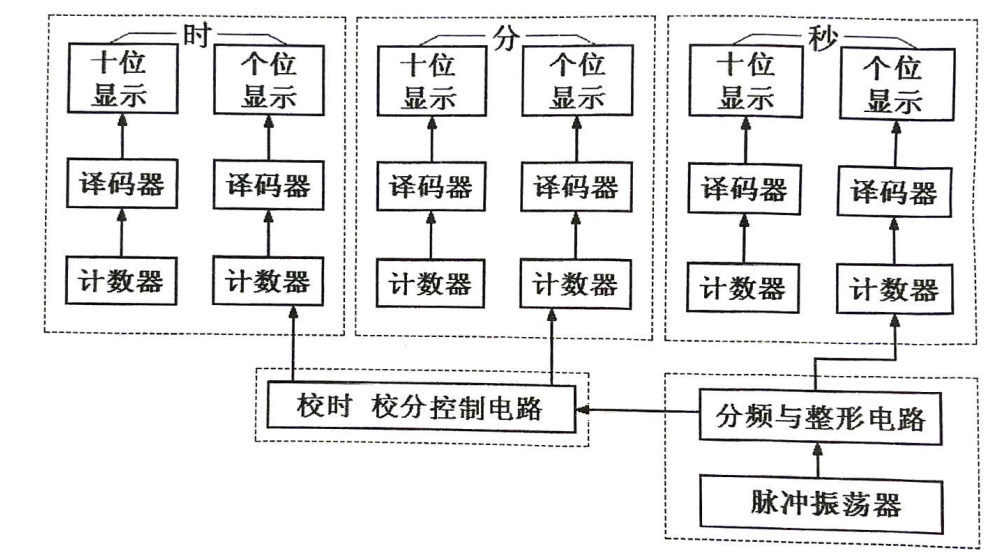
\includegraphics[width=10cm]{2.1.png}
    \end{figure}

    振荡器是整个数字中的核心,他的稳定度和频率的精准度决定了数字钟计时的准确性,是影响数字钟质量的决定性因素,其产生的时钟信号经过分频器产生秒信号,输入到计数器进行计数。

    数字钟的计数电路可用2个60进制和1个24禁止实现,60进制计数器由1个10禁止计数器和一个6进制计数器组成,分别对应个位和十位,24进制计数器作为时计数器。计数器由六片74LS90组成,可用反馈归零法设计。

    由于连接方式不同,集成异步计数器芯片74Ls90可以实现四种不同的逻辑功能,有二进制加法计数器,异步五进制加法计数器,十进制加法计数器和异步清零,置九功能等,具体实现如下表所示:
    
    \begin{figure}[htbp]
        \centering
        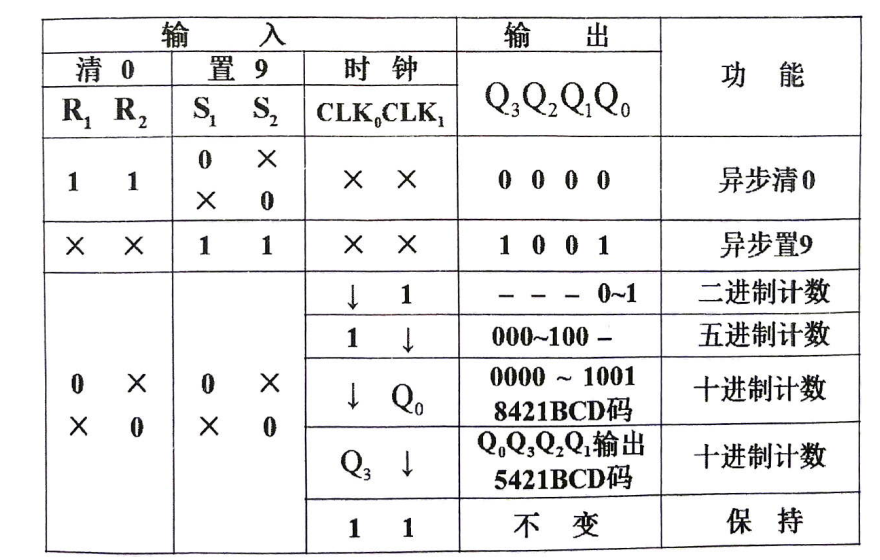
\includegraphics[width=10cm]{2.2.png}
    \end{figure}

    实验中可设有两个快速校准电路,由SR锁存器和与非门组成。正常工作时两个开关合到$S'_D$端,SR锁存器置1,分,时脉冲通过。当开关合到$R'_D$端时,SR锁存器置0,正常计数不能通过,而秒脉冲通过,使得分,时计数器变成了秒计数器可以快速校准。电路图如下:
    
    \begin{figure}[htbp]
        \centering
        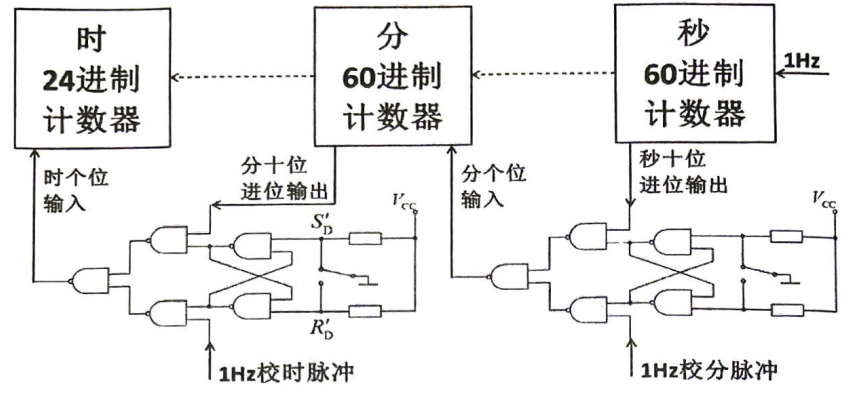
\includegraphics[width=\textwidth]{2.3.png}
    \end{figure}

    
    \section*{第三部分 \quad 实验内容}
    \begin{enumerate}
        \item 试用74LS90设计数字钟用24进制和60进制计数器
        \item 在实验内容1的基础上增加校时电路
        \item 在实验内容1的基础上实现报时功能
    \end{enumerate}

    完整的设计电路如图所示:

    \begin{minipage}[c]{\textwidth}
        \centering
        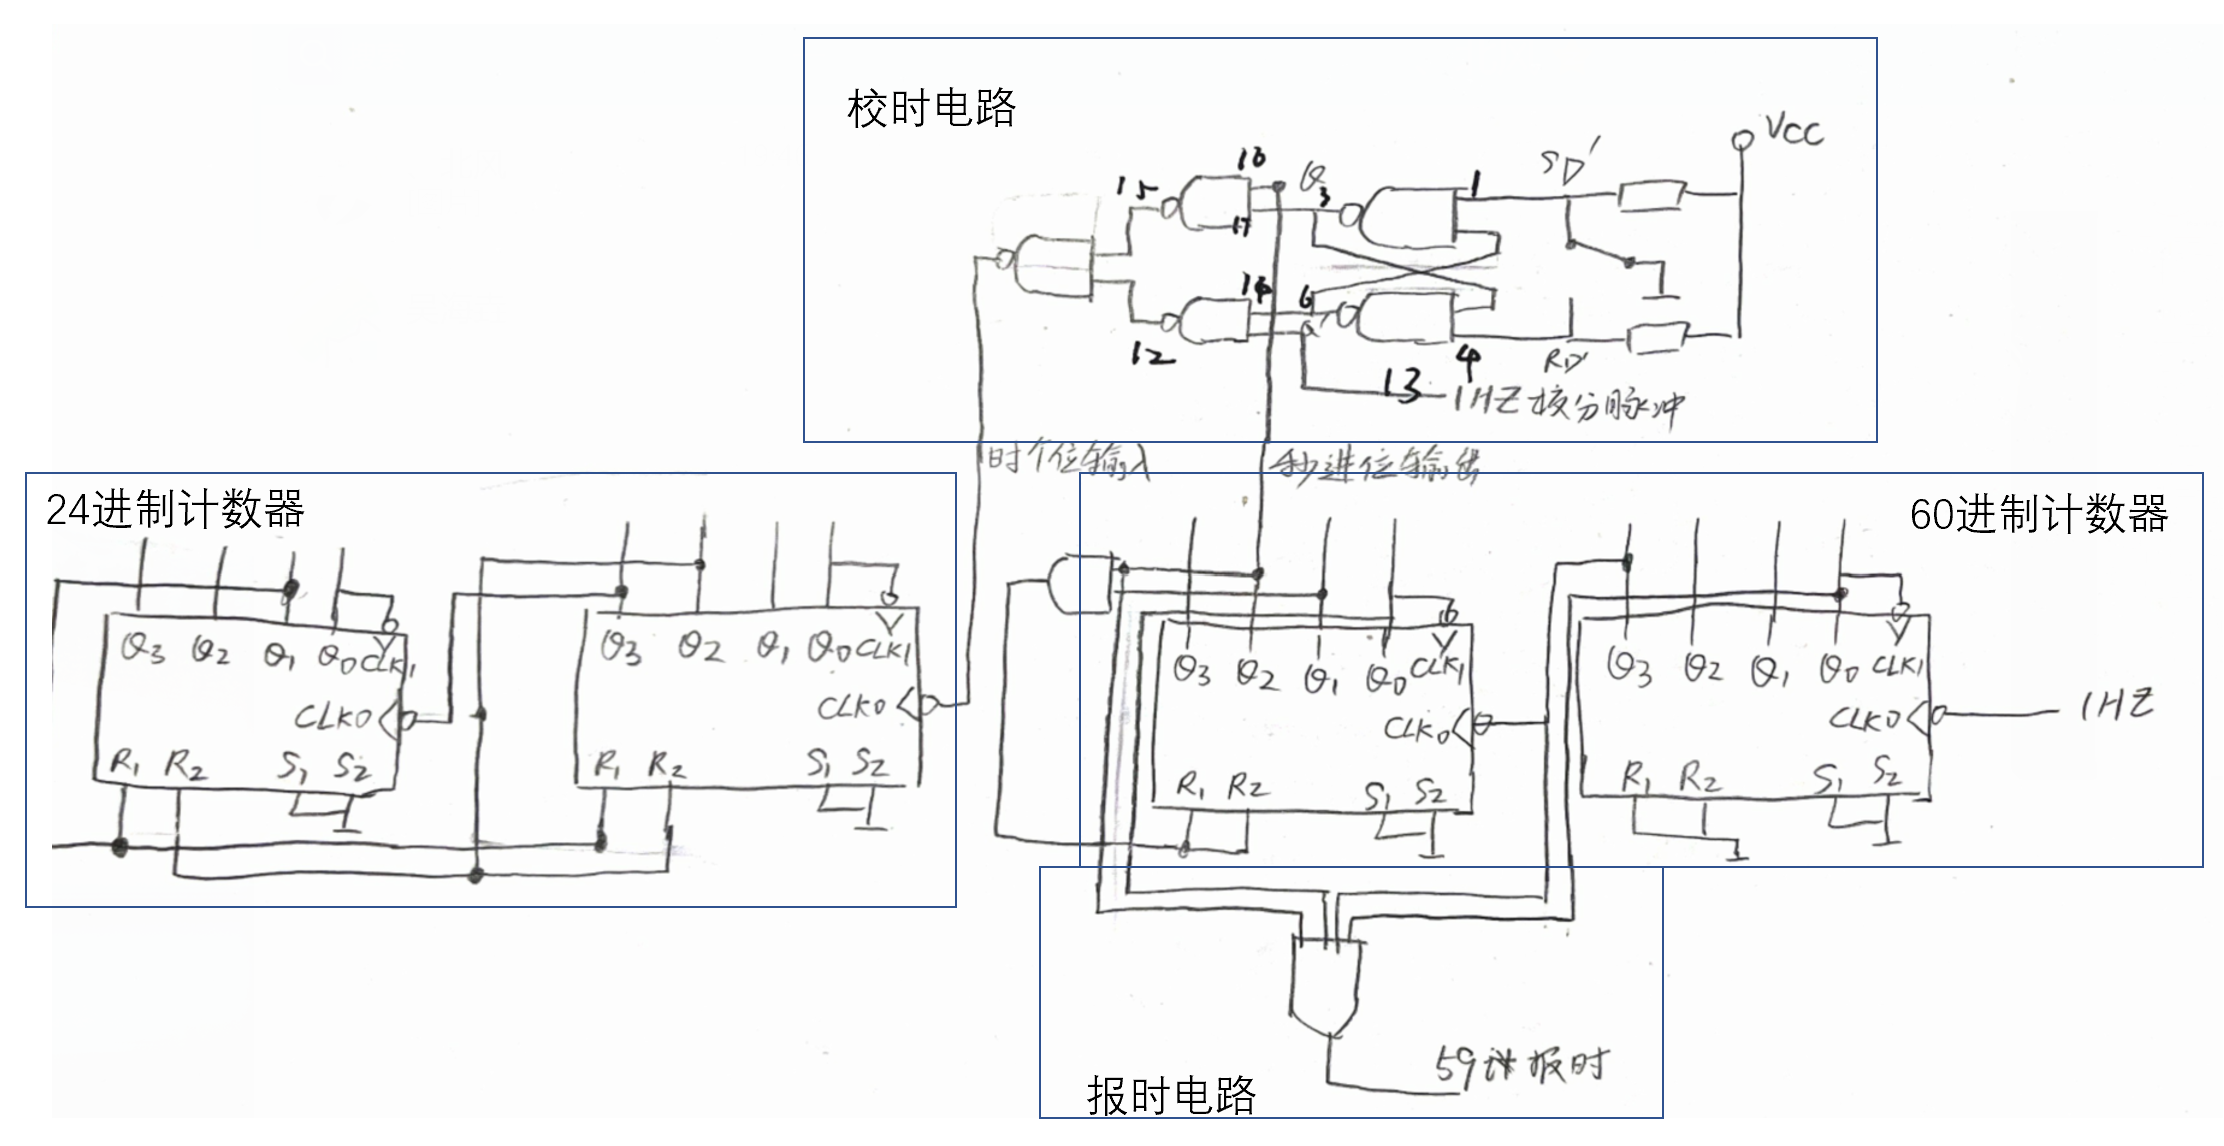
\includegraphics[width=\linewidth]{graph.png} 
    \end{minipage}

    \begin{enumerate}
        \item 各使用两片74LS90搭建24进制计数器和60进制计数器。60进制计数器输入频率为1Hz的时钟信号,采用十位异步置零的方式,实现60进制计数。输出接入校时电路的输入端。24进制计数器输入为校时电路的输出信号,采用整体异步置零的方式,实现24进制计数。
        \item 校时电路参考实验原理。当按下按钮时,时位(24进制计数器)输入1Hz的时钟信号,实现校时。按钮未按下时则正常接收来自低位的信号。
        \item 报时电路如图所示,通过与门,使得电路在秒位(60进制计数器)计数到59时,产生报时信号。
    \end{enumerate}
    
    \newpage
    \section*{第四部分 \quad 思考题}
    \subsection*{1.试用555设计秒脉冲器}
    设计电路图如下:
    \begin{figure}[htbp]
        \centering
        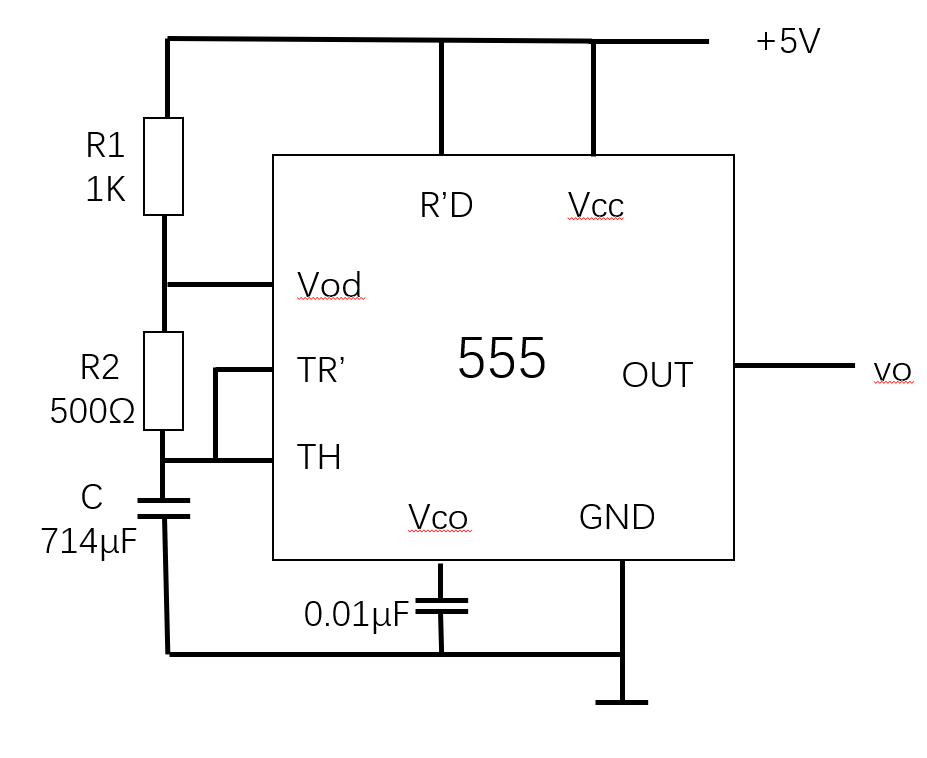
\includegraphics[width=9cm]{4.1.png}
    \end{figure}

    通过前备知识用555搭建多谐振荡器,注意到振荡器的周期和占空比与所连电阻,电容相关,因此为了输出所想要的脉冲,要设计计算其数值,实现振荡

    \subsection*{2.画出完整的数字钟逻辑电路图,并说明各部分的原理与功能}
     如实验内容所示。

     \subsection*{3.设计一个具有整点报时功能的电路}
       \begin{minipage}[c]{\textwidth}
        \centering
        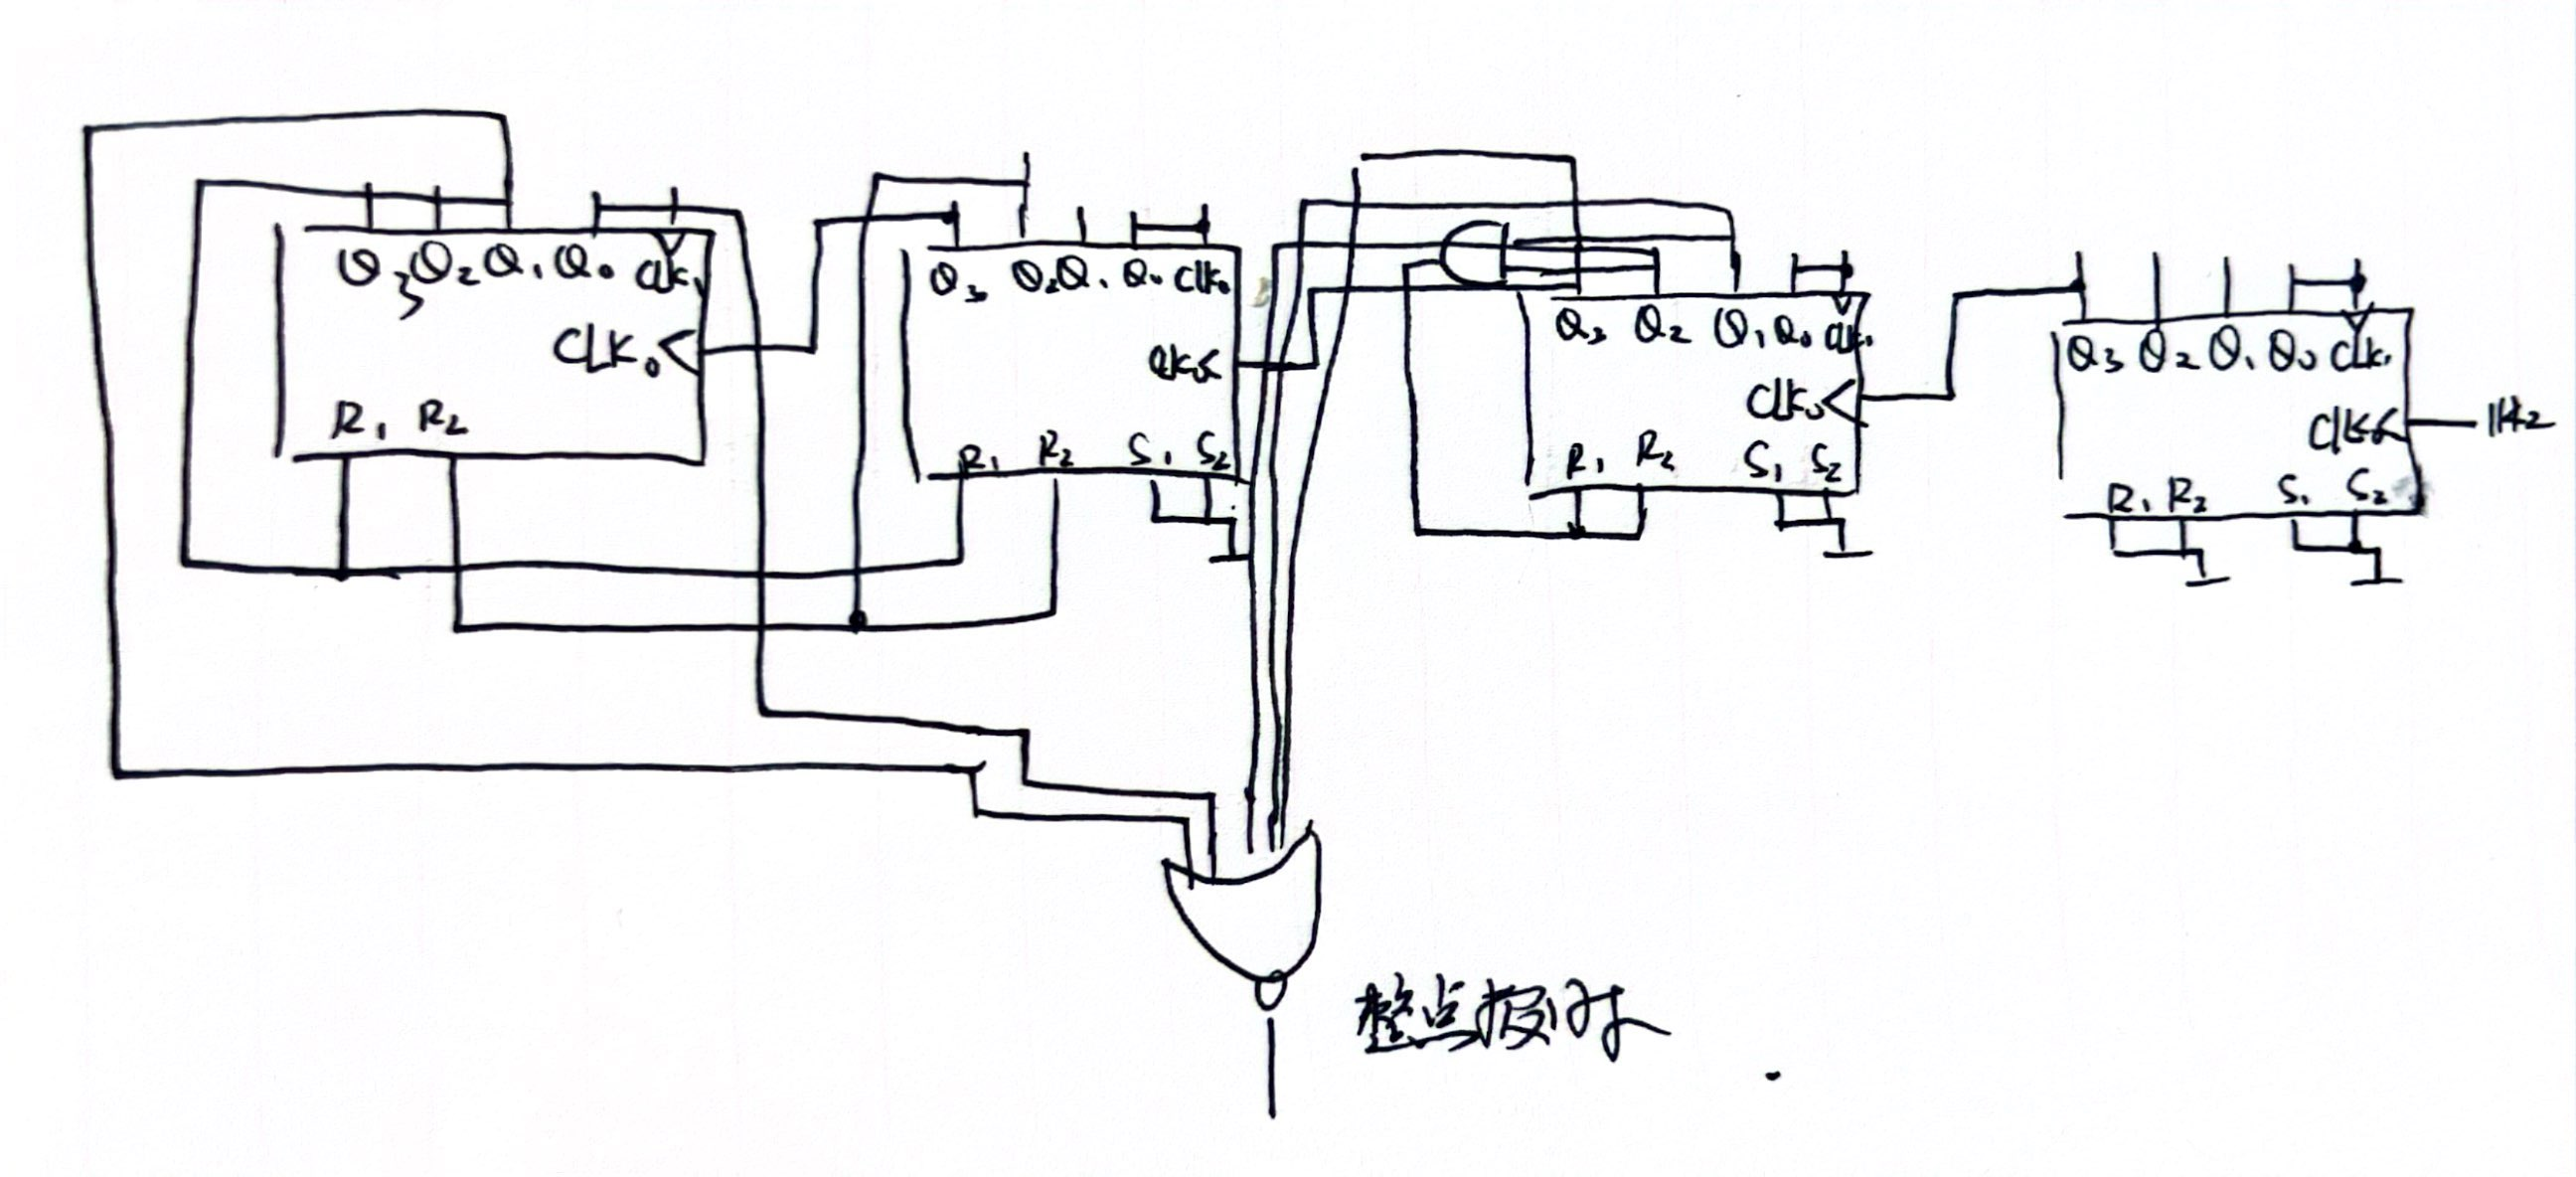
\includegraphics[width=\linewidth]{4.2.png} 
    \end{minipage}

    整体设计思路与实验内容类似,但是注意的是判断报时的条件不同,需要是准点时刻

\end{document}